\documentclass[12pt]{article}
\usepackage{hyperref}
\usepackage{longtable}
\usepackage{lscape}
\usepackage{booktabs}
\usepackage{makecell}
\usepackage{graphicx}
\usepackage[margin=1in]{geometry}
\usepackage{xspace}
\newcommand{\varn}[1]{\ifmmode\text{\textit{#1}}\else\textit{#1}\fi\xspace}
\newcommand{\Intercept}{\varn{Intercept}}
\newcommand{\Province}{\varn{Province}}
\newcommand{\QOESpend}{\varn{QOE.Spend}}
\newcommand{\QOESpendRatio}{\varn{QOE.Spend.Ratio}}
\newcommand{\QOESpendingPH}{\varn{QOE.Spend.PerHour}}
\newcommand{\QOESpendingph}{\varn{QOE.Spend.PerHour}}
\newcommand{\QOESpending}{\varn{QOE.Spend}}
\newcommand{\GDPPrimary}{\varn{GDP.Primary}}
\newcommand{\CPI}{\varn{CPI}}
\newcommand{\NumEnterprise}{\varn{Num.Enterprise}}
\newcommand{\TotalIncome}{\varn{Total.Income}}
\newcommand{\TotalSpending}{\varn{Total.Spending}}
\newcommand{\Engel}{\varn{Engel}}
\newcommand{\Pop}{\varn{Population}}
\newcommand{\PopHighEduMale}{\varn{Pop.High.Edu.Male}}
\newcommand{\PopHighEduFemale}{\varn{Pop.High.Edu.Female}}
\newcommand{\HighEducated}{\varn{Pop.High.Educated}}
\newcommand{\Gini}{\varn{Gini}}
\newcommand{\UrbanSpendTotal}{\varn{Urban.Spend.Total}}
\newcommand{\UrbanSpendFood}{\varn{Urban.Spend.Food}}
\newcommand{\Asset}{\varn{Asset}}
\newcommand{\Debt}{\varn{Debt}}
\newcommand{\HighEdu}{\varn{High.Edu.Parent}}
\newcommand{\Age}{\varn{Age}}
\newcommand{\QOETime}{\varn{QOE.Time}}
\newcommand{\prov}{\varn{prov}}
\newcommand{\geom}{\varn{geom}}
\newcommand{\GenderMale}{\varn{Gender.Male}}
\newcommand{\RegionUrban}{\varn{Region.Urban}}
\newcommand{\CultCentCountTotal}{\varn{Youth.Palace.Count}}
\newcommand{\UniversityRecruitRatio}{\varn{University.Recruit.Ratio}}
\newcommand{\GeneralEduBudget}{\varn{General.Edu.Budget}}
\newcommand{\NationalFiscalExpenditure}{\varn{National.Fiscal.Expenditure}}

\begin{document}

\def\spacingset#1{\renewcommand{\baselinestretch}%
{#1}\small\normalsize} \spacingset{1}

\title{Supplemental Materials for ``Testing Spatial Heterogeneity in Hierarchical and Geographically Weighted Regression: Theory, Simulation, and a Study of Extracurricular Education in China''}
\author{}

\maketitle

\spacingset{1.8}

\section{Further details on the QOE results}\label{app:further-details}

Estimate values for GLSW and SLR effects of the model in the main text are shown in \autoref{tbl:model-coef-glsw-slr}.
Significance of each estimate is evaluated according to the t-test and is shown after the estimate using significance codes.

The alternative model is summarised in \autoref{tbl:modelratio-summary}, showing estimated values, standard errors and results of hypothesis tests for fixed, GLSW, and SLR effects.
Estimates for GLSW and SLR effects of the alternative model are shown in Table \autoref{tbl:modelratio-coef-glsw-slr} are visualised in \autoref{fig:modelratio-coef-glsw-slr}.

\begin{landscape}
\begin{small}
  \centering
  \begin{longtable}{lrrrrrrrrr}
    \caption[Values of GLSW and SLR effects and the corresponding variances in each province from the main model.]{Values of GLSW and SLR effects and the corresponding variances in each province from the main model.}
    \label{tbl:model-coef-glsw-slr}\\
    \toprule
    \Province & \Intercept & {\itshape\makecell[r]{GDP.\\Primary}} & \Engel & \CPI & \Gini & {\itshape\makecell[r]{University.\\Recruit.\\Ratio}} & {\itshape\makecell[r]{General.\\Edu.\\Budget}} & {\itshape\makecell[r]{Pop.\\High.\\Educated}} & {\itshape\makecell[r]{Region.\\Urban}} \\\midrule
    \endfirsthead
    \multicolumn{10}{r}{(continued)}\\
    \toprule
    \Province & \Intercept & {\itshape\makecell[r]{GDP.\\Primary}} & \Engel & \CPI & \Gini & {\itshape\makecell[r]{University.\\Recruit.\\Ratio}} & {\itshape\makecell[r]{General.\\Edu.\\Budget}} & {\itshape\makecell[r]{Pop.\\High.\\Educated}} & {\itshape\makecell[r]{Region.\\Urban}} \\\midrule
    \endhead
    \bottomrule
    \multicolumn{10}{r}{(continues on the next page...)}\\
    \endfoot
    \bottomrule
    \multicolumn{10}{l}{Significance code: 0 `***' 0.001 `**' 0.01 `*' 0.05 `.' 0.1 ` ' 1}\\
    \endlastfoot
    Shanghai & 8.282 & \makecell[r]{0.921\\(0.889)} & \makecell[r]{0.938*\\(0.395)} & \makecell[r]{0.060\\(0.563)} & \makecell[r]{-0.475\\(0.548)} & \makecell[r]{-22.053*\\(10.825)} & \makecell[r]{4.642***\\(0.878)} & \makecell[r]{4.162**\\(1.552)} & 0.395 \\
    Yunnan & -0.526 & \makecell[r]{1.447\\(1.760)} & \makecell[r]{-0.609\\(0.372)} & \makecell[r]{-0.392\\(0.441)} & \makecell[r]{0.235\\(0.531)} & \makecell[r]{7.707\\(14.091)} & \makecell[r]{3.810***\\(1.131)} & \makecell[r]{2.273\\(1.792)} & 0.313 \\
    Neimenggu & 3.176 & \makecell[r]{-0.149\\(0.911)} & \makecell[r]{1.094**\\(0.409)} & \makecell[r]{0.627\\(0.574)} & \makecell[r]{-1.295**\\(0.466)} & \makecell[r]{-11.205\\(7.756)} & \makecell[r]{5.127***\\(0.957)} & \makecell[r]{1.856\\(1.205)} & 0.662 \\
    Beijing & 3.094 & \makecell[r]{-0.221\\(0.940)} & \makecell[r]{1.116**\\(0.396)} & \makecell[r]{0.421\\(0.562)} & \makecell[r]{-0.744\\(0.476)} & \makecell[r]{-8.442\\(7.826)} & \makecell[r]{5.479***\\(1.001)} & \makecell[r]{1.480\\(1.186)} & 0.569 \\
    Jilin & 4.530 & \makecell[r]{-0.157\\(0.865)} & \makecell[r]{0.890*\\(0.385)} & \makecell[r]{0.617\\(0.582)} & \makecell[r]{-0.626\\(0.694)} & \makecell[r]{-8.464\\(8.322)} & \makecell[r]{5.606***\\(0.964)} & \makecell[r]{1.556\\(1.265)} & -0.026 \\
    Sichuan & -0.037 & \makecell[r]{3.040.\\(1.667)} & \makecell[r]{-0.528\\(0.380)} & \makecell[r]{-0.577\\(0.446)} & \makecell[r]{-0.475\\(0.523)} & \makecell[r]{7.226\\(14.221)} & \makecell[r]{2.161*\\(1.077)} & \makecell[r]{1.500\\(1.808)} & 0.681 \\
    Tianjin & 2.334 & \makecell[r]{-0.127\\(0.911)} & \makecell[r]{1.067**\\(0.392)} & \makecell[r]{0.294\\(0.568)} & \makecell[r]{-0.489\\(0.512)} & \makecell[r]{-6.057\\(8.022)} & \makecell[r]{5.579***\\(0.992)} & \makecell[r]{1.256\\(1.195)} & 0.534 \\
    Ningxia & -6.691 & \makecell[r]{3.233***\\(0.903)} & \makecell[r]{-0.238\\(0.512)} & \makecell[r]{-0.436\\(0.468)} & \makecell[r]{-1.010.\\(0.579)} & \makecell[r]{26.738**\\(9.007)} & \makecell[r]{0.442\\(0.963)} & \makecell[r]{-2.216\\(1.389)} & 0.071 \\
    Anhui & 10.598 & \makecell[r]{2.576*\\(1.151)} & \makecell[r]{1.041**\\(0.404)} & \makecell[r]{0.112\\(0.551)} & \makecell[r]{-0.858\\(0.578)} & \makecell[r]{-28.879*\\(12.163)} & \makecell[r]{3.064*\\(1.208)} & \makecell[r]{6.275**\\(2.066)} & 0.989 \\
    Shandong & 3.289 & \makecell[r]{-0.212\\(0.900)} & \makecell[r]{1.126**\\(0.412)} & \makecell[r]{0.191\\(0.580)} & \makecell[r]{-0.241\\(0.555)} & \makecell[r]{-8.708\\(9.515)} & \makecell[r]{6.147***\\(1.060)} & \makecell[r]{1.720\\(1.309)} & 0.979 \\
    Shanxi & 3.936 & \makecell[r]{-0.540\\(1.239)} & \makecell[r]{1.275**\\(0.484)} & \makecell[r]{0.805\\(0.609)} & \makecell[r]{-0.992*\\(0.494)} & \makecell[r]{-10.532\\(9.744)} & \makecell[r]{5.480***\\(1.309)} & \makecell[r]{1.619\\(1.413)} & 0.433 \\
    Guangdong & -3.986 & \makecell[r]{4.412***\\(0.922)} & \makecell[r]{-0.818\\(0.499)} & \makecell[r]{-2.735***\\(0.689)} & \makecell[r]{0.275\\(0.428)} & \makecell[r]{18.971\\(13.188)} & \makecell[r]{2.270**\\(0.762)} & \makecell[r]{0.820\\(2.306)} & 0.931 \\
    Guangxi & -4.418 & \makecell[r]{2.394\\(1.538)} & \makecell[r]{-0.684\\(0.477)} & \makecell[r]{-1.686**\\(0.607)} & \makecell[r]{0.249\\(0.491)} & \makecell[r]{19.461\\(12.873)} & \makecell[r]{3.438**\\(1.045)} & \makecell[r]{0.476\\(1.886)} & 0.145 \\
    Jiangsu & 7.387 & \makecell[r]{0.570\\(0.906)} & \makecell[r]{1.112**\\(0.404)} & \makecell[r]{0.168\\(0.563)} & \makecell[r]{-0.396\\(0.524)} & \makecell[r]{-20.718*\\(10.510)} & \makecell[r]{5.315***\\(1.023)} & \makecell[r]{3.886*\\(1.530)} & 0.104 \\
    Jiangxi & 4.239 & \makecell[r]{4.264***\\(1.008)} & \makecell[r]{-0.244\\(0.416)} & \makecell[r]{-1.646**\\(0.569)} & \makecell[r]{0.070\\(0.463)} & \makecell[r]{-4.360\\(11.269)} & \makecell[r]{1.884*\\(0.921)} & \makecell[r]{4.535*\\(2.105)} & 0.426 \\
    Hebei & 2.633 & \makecell[r]{-0.338\\(0.961)} & \makecell[r]{1.176**\\(0.407)} & \makecell[r]{0.483\\(0.560)} & \makecell[r]{-0.805.\\(0.468)} & \makecell[r]{-10.431\\(8.198)} & \makecell[r]{5.647***\\(1.039)} & \makecell[r]{1.706\\(1.203)} & 0.504 \\
    Henan & 6.048 & \makecell[r]{1.478\\(1.258)} & \makecell[r]{1.033*\\(0.437)} & \makecell[r]{0.343\\(0.555)} & \makecell[r]{-0.848*\\(0.423)} & \makecell[r]{-14.396\\(8.768)} & \makecell[r]{4.023**\\(1.230)} & \makecell[r]{3.360*\\(1.472)} & 0.282 \\
    Zhejiang & 15.272 & \makecell[r]{3.254**\\(1.191)} & \makecell[r]{0.486\\(0.468)} & \makecell[r]{-0.082\\(0.599)} & \makecell[r]{-0.699\\(0.689)} & \makecell[r]{-34.827*\\(13.725)} & \makecell[r]{1.725\\(1.156)} & \makecell[r]{7.723***\\(2.222)} & 0.226 \\
    Hainan & -6.914 & \makecell[r]{3.388***\\(1.005)} & \makecell[r]{-0.660\\(0.527)} & \makecell[r]{-2.453***\\(0.676)} & \makecell[r]{0.129\\(0.521)} & \makecell[r]{27.229.\\(14.320)} & \makecell[r]{3.134***\\(0.743)} & \makecell[r]{-1.149\\(2.423)} & 0.295 \\
    Hubei & -0.005 & \makecell[r]{3.421*\\(1.369)} & \makecell[r]{0.366\\(0.451)} & \makecell[r]{-0.900\\(0.597)} & \makecell[r]{-1.735*\\(0.684)} & \makecell[r]{9.884\\(12.048)} & \makecell[r]{1.378\\(1.132)} & \makecell[r]{1.327\\(2.014)} & 0.227 \\
    Hunan & -6.445 & \makecell[r]{5.193**\\(1.597)} & \makecell[r]{-0.661\\(0.523)} & \makecell[r]{-3.046***\\(0.837)} & \makecell[r]{-0.374\\(0.452)} & \makecell[r]{26.224.\\(14.893)} & \makecell[r]{1.881\\(1.146)} & \makecell[r]{-0.474\\(2.384)} & 0.339 \\
    Gansu & -5.565 & \makecell[r]{3.988***\\(1.037)} & \makecell[r]{0.101\\(0.640)} & \makecell[r]{-0.900\\(0.631)} & \makecell[r]{-1.821.\\(0.929)} & \makecell[r]{24.276*\\(10.977)} & \makecell[r]{-0.084\\(1.056)} & \makecell[r]{-1.607\\(1.630)} & 1.410 \\
    Fujian & 5.806 & \makecell[r]{4.110***\\(1.061)} & \makecell[r]{-0.486\\(0.479)} & \makecell[r]{-1.685**\\(0.598)} & \makecell[r]{0.538\\(0.441)} & \makecell[r]{-7.072\\(11.887)} & \makecell[r]{1.942*\\(0.930)} & \makecell[r]{5.272*\\(2.186)} & 0.360 \\
    Guizhou & -2.476 & \makecell[r]{1.403\\(1.927)} & \makecell[r]{-0.648\\(0.448)} & \makecell[r]{-0.737\\(0.703)} & \makecell[r]{0.179\\(0.521)} & \makecell[r]{12.822\\(13.395)} & \makecell[r]{3.759**\\(1.312)} & \makecell[r]{1.492\\(1.760)} & 0.007 \\
    Liaoning & 2.442 & \makecell[r]{-0.081\\(0.856)} & \makecell[r]{0.928*\\(0.379)} & \makecell[r]{0.420\\(0.558)} & \makecell[r]{-0.402\\(0.656)} & \makecell[r]{-5.493\\(7.991)} & \makecell[r]{5.638***\\(0.953)} & \makecell[r]{1.246\\(1.228)} & 0.527 \\
    Chongqing & -1.290 & \makecell[r]{2.476\\(1.847)} & \makecell[r]{0.030\\(0.479)} & \makecell[r]{-0.830\\(0.743)} & \makecell[r]{-1.687*\\(0.698)} & \makecell[r]{15.966\\(13.090)} & \makecell[r]{2.217.\\(1.320)} & \makecell[r]{0.869\\(1.700)} & 1.197 \\
    Shaanxi & -5.366 & \makecell[r]{2.741**\\(0.919)} & \makecell[r]{-0.036\\(0.455)} & \makecell[r]{-0.226\\(0.553)} & \makecell[r]{-0.953.\\(0.512)} & \makecell[r]{19.892*\\(9.993)} & \makecell[r]{1.164\\(1.024)} & \makecell[r]{-1.438\\(1.625)} & 0.150 \\
    Qinghai & -3.737 & \makecell[r]{4.072**\\(1.344)} & \makecell[r]{0.246\\(0.697)} & \makecell[r]{-1.164.\\(0.679)} & \makecell[r]{-2.416*\\(1.171)} & \makecell[r]{22.334.\\(13.265)} & \makecell[r]{0.093\\(1.231)} & \makecell[r]{-0.798\\(2.016)} & 0.368 \\
    Heilongjiang & 2.296 & \makecell[r]{0.025\\(0.889)} & \makecell[r]{0.813*\\(0.412)} & \makecell[r]{0.781\\(0.615)} & \makecell[r]{-0.870\\(0.734)} & \makecell[r]{-8.727\\(8.419)} & \makecell[r]{5.365***\\(0.977)} & \makecell[r]{1.693\\(1.289)} & 0.620 \\
  \end{longtable}

  \begin{longtable}{lrrlrrlr}
    \caption{Summary of the alternative model.}
    \label{tbl:modelratio-summary}\\
    \toprule
    Fixed               & \makecell[r]{Estimated\\(Std. Err.)} & \makecell[r]{$t$-value\\($p$-value)} & GLSW                    & \makecell[r]{Mean Est.\\(Mean S.E.)} & \makecell[r]{$F$-value\\($p$-value)} & SLR          & \makecell[r]{Mean Est.\\(Std. Err.)} \\
    \midrule
    \endfirsthead
    \multicolumn{8}{r}{(continued)}\\
    \toprule
    Fixed               & \makecell[r]{Estimated\\(Std. Err.)} & \makecell[r]{$t$-value\\($p$-value)} & GLSW                    & \makecell[r]{Mean Est.\\(Mean S.E.)} & \makecell[r]{$F$-value\\($p$-value)} & SLR          & \makecell[r]{Mean Est.\\(Std. Err.)} \\
    \midrule
    \endhead
    \bottomrule
    \multicolumn{8}{r}{(continues on the next page...)}\\
    \endfoot
    \bottomrule
    \multicolumn{7}{l}{Significance codes: `***' 0.001 `**' 0.01 `*' 0.05 `.' 0.1 ` '} \\
    \endlastfoot
    \Intercept          & \makecell[r]{-11.210\\(0.228)}       & \makecell[r]{49.092***\\(0.000)}   & \Intercept              & \makecell[r]{4.083\\(6.205)}         & \makecell[r]{3.736***\\(0.000)}    & \Intercept   & \makecell[r]{0.000\\(1.064)}         \\
    \NumEnterprise      & \makecell[r]{-6.752\\(0.565)}        & \makecell[r]{11.944***\\(0.000)}   & \GDPPrimary             & \makecell[r]{3.008\\(1.321)}         & \makecell[r]{5.491***\\(0.000)}    & \RegionUrban & \makecell[r]{-0.000\\(1.064)}        \\
    \CultCentCountTotal & \makecell[r]{0.511\\(0.612)}         & \makecell[r]{0.836\\(0.403)}       & \Engel                  & \makecell[r]{12.603\\(18.087)}       & \makecell[r]{10.940***\\(0.000)}   &              &                                      \\
    \TotalIncome        & \makecell[r]{0.025\\(0.022)}         & \makecell[r]{1.122\\(0.262)}       & \CPI                    & \makecell[r]{-0.636\\(0.670)}        & \makecell[r]{12.825***\\(0.000)}   &              &                                      \\
    \Asset              & \makecell[r]{-0.025\\(0.027)}        & \makecell[r]{0.935\\(0.350)}       & \Gini                   & \makecell[r]{-6.303\\(4.263)}        & \makecell[r]{2.114*\\(0.015)}      &              &                                      \\
    \Debt               & \makecell[r]{-0.035\\(0.022)}        & \makecell[r]{1.563\\(0.118)}       & \UniversityRecruitRatio & \makecell[r]{2.027\\(12.566)}        & \makecell[r]{6.652***\\(0.000)}    &              &                                      \\
    \HighEdu            & \makecell[r]{0.209\\(0.050)}         & \makecell[r]{4.154***\\(0.000)}    & \GeneralEduBudget       & \makecell[r]{3.677\\(1.196)}         & \makecell[r]{6.239***\\(0.000)}    &              &                                      \\
    \GenderMale         & \makecell[r]{-0.157\\(0.044)}        & \makecell[r]{3.602***\\(0.000)}    & \HighEducated           & \makecell[r]{2.213\\(1.923)}         & \makecell[r]{4.220***\\(0.000)}    &              &                                      \\
    \RegionUrban        & \makecell[r]{0.465\\(0.218)}         & \makecell[r]{2.130*\\(0.033)}      &                         &                                      &                                    &              &                                      \\
    \Age                & \makecell[r]{-0.109\\(0.022)}        & \makecell[r]{4.949***\\(0.000)}    &                         &                                      &                                    &              &                                      \\
  \end{longtable}

  \begin{longtable}{lrrrrrrrrr}
    \caption{Values of GLSW and SLR effects in each province from the alternative model.}
    \label{tbl:modelratio-coef-glsw-slr}\\
    \toprule
    \Province & \Intercept & {\itshape\makecell[r]{GDP.\\Primary}} & \Engel & \CPI & \Gini & {\itshape\makecell[r]{University.\\Recruit.\\Ratio}} & {\itshape\makecell[r]{General.\\Edu.\\Budget}} & {\itshape\makecell[r]{Pop.\\High.\\Educated}} & {\itshape\makecell[r]{Region.\\Urban}} \\\midrule
    \endfirsthead
    \multicolumn{10}{r}{(continued)}\\
    \toprule
    \Province & \Intercept & {\itshape\makecell[r]{GDP.\\Primary}} & \Engel & \CPI & \Gini & {\itshape\makecell[r]{University.\\Recruit.\\Ratio}} & {\itshape\makecell[r]{General.\\Edu.\\Budget}} & {\itshape\makecell[r]{Pop.\\High.\\Educated}} & {\itshape\makecell[r]{Region.\\Urban}} \\\midrule
    \endhead
    \bottomrule
    \multicolumn{10}{r}{(continues on the next page...)}\\
    \endfoot
    \bottomrule
    \multicolumn{10}{l}{Significance code: 0 `***' 0.001 `**' 0.01 `*' 0.05 `.' 0.1 ` ' 1}\\
    \endlastfoot
    Shanghai & -9.130 & \makecell[r]{1.805.\\(1.011)} & \makecell[r]{0.144\\(0.629)} & \makecell[r]{47.173**\\(16.014)} & \makecell[r]{-6.313\\(4.095)} & \makecell[r]{-26.027*\\(12.164)} & \makecell[r]{5.259***\\(1.002)} & \makecell[r]{5.449**\\(1.734)} & 0.312 \\
    Yunnan & 6.863 & \makecell[r]{2.225\\(1.974)} & \makecell[r]{-0.753\\(0.491)} & \makecell[r]{-46.581**\\(14.556)} & \makecell[r]{1.782\\(3.815)} & \makecell[r]{13.519\\(15.910)} & \makecell[r]{4.507***\\(1.267)} & \makecell[r]{3.022\\(2.032)} & 0.907 \\
    Neimenggu & -13.398 & \makecell[r]{0.659\\(1.034)} & \makecell[r]{1.003\\(0.637)} & \makecell[r]{54.737***\\(16.323)} & \makecell[r]{-12.331***\\(3.345)} & \makecell[r]{-15.839.\\(8.858)} & \makecell[r]{5.971***\\(1.101)} & \makecell[r]{3.438*\\(1.352)} & -0.377 \\
    Beijing & -15.952 & \makecell[r]{0.589\\(1.049)} & \makecell[r]{0.718\\(0.624)} & \makecell[r]{55.685***\\(15.710)} & \makecell[r]{-9.189**\\(3.448)} & \makecell[r]{-12.589\\(8.811)} & \makecell[r]{6.216***\\(1.122)} & \makecell[r]{2.899*\\(1.331)} & 0.517 \\
    Jilin & -9.934 & \makecell[r]{0.448\\(0.972)} & \makecell[r]{1.036\\(0.655)} & \makecell[r]{46.493**\\(15.333)} & \makecell[r]{-9.907.\\(5.380)} & \makecell[r]{-15.838.\\(9.547)} & \makecell[r]{6.323***\\(1.107)} & \makecell[r]{3.145*\\(1.453)} & 0.147 \\
    Sichuan & 7.718 & \makecell[r]{4.619*\\(1.867)} & \makecell[r]{-0.970.\\(0.498)} & \makecell[r]{-38.295*\\(14.926)} & \makecell[r]{-3.140\\(3.765)} & \makecell[r]{11.354\\(16.029)} & \makecell[r]{2.043.\\(1.208)} & \makecell[r]{1.908\\(2.043)} & 0.694 \\
    Tianjin & -16.928 & \makecell[r]{0.657\\(1.007)} & \makecell[r]{0.555\\(0.631)} & \makecell[r]{54.122***\\(15.455)} & \makecell[r]{-7.398*\\(3.701)} & \makecell[r]{-9.836\\(8.961)} & \makecell[r]{6.302***\\(1.100)} & \makecell[r]{2.568.\\(1.338)} & 0.713 \\
    Ningxia & -7.368 & \makecell[r]{4.535***\\(1.015)} & \makecell[r]{-0.562\\(0.522)} & \makecell[r]{-18.489\\(20.575)} & \makecell[r]{-6.924.\\(4.184)} & \makecell[r]{40.831***\\(10.024)} & \makecell[r]{-0.052\\(1.074)} & \makecell[r]{-3.433*\\(1.556)} & 0.300 \\
    Anhui & -7.168 & \makecell[r]{3.696**\\(1.254)} & \makecell[r]{0.192\\(0.613)} & \makecell[r]{51.787**\\(15.866)} & \makecell[r]{-9.267*\\(4.162)} & \makecell[r]{-31.648*\\(13.167)} & \makecell[r]{3.459**\\(1.318)} & \makecell[r]{7.552***\\(2.238)} & 0.313 \\
    Shandong & -18.553 & \makecell[r]{0.543\\(0.991)} & \makecell[r]{0.322\\(0.650)} & \makecell[r]{56.745***\\(16.198)} & \makecell[r]{-5.151\\(4.091)} & \makecell[r]{-10.749\\(10.644)} & \makecell[r]{6.920***\\(1.172)} & \makecell[r]{2.714.\\(1.466)} & 0.814 \\
    Shanxi & -16.940 & \makecell[r]{0.381\\(1.390)} & \makecell[r]{1.014\\(0.674)} & \makecell[r]{63.894***\\(19.018)} & \makecell[r]{-10.817**\\(3.535)} & \makecell[r]{-14.385\\(10.844)} & \makecell[r]{6.179***\\(1.465)} & \makecell[r]{3.062.\\(1.587)} & 0.113 \\
    Guangdong & 4.142 & \makecell[r]{6.779***\\(1.064)} & \makecell[r]{-4.414***\\(0.810)} & \makecell[r]{-58.760**\\(20.791)} & \makecell[r]{0.835\\(3.276)} & \makecell[r]{38.716*\\(15.782)} & \makecell[r]{2.188*\\(0.905)} & \makecell[r]{-0.736\\(2.758)} & 0.537 \\
    Guangxi & 1.431 & \makecell[r]{3.846*\\(1.951)} & \makecell[r]{-2.934***\\(0.708)} & \makecell[r]{-52.974**\\(18.922)} & \makecell[r]{0.547\\(3.678)} & \makecell[r]{38.937*\\(16.057)} & \makecell[r]{3.913**\\(1.310)} & \makecell[r]{-1.001\\(2.198)} & 0.799 \\
    Jiangsu & -13.791 & \makecell[r]{1.420\\(1.003)} & \makecell[r]{0.240\\(0.626)} & \makecell[r]{55.459***\\(15.895)} & \makecell[r]{-5.871\\(3.837)} & \makecell[r]{-22.798*\\(11.599)} & \makecell[r]{6.032***\\(1.132)} & \makecell[r]{4.902**\\(1.687)} & -0.012 \\
    Jiangxi & 2.339 & \makecell[r]{6.131***\\(1.132)} & \makecell[r]{-2.324***\\(0.637)} & \makecell[r]{-14.465\\(16.770)} & \makecell[r]{-1.413\\(3.521)} & \makecell[r]{2.041\\(12.800)} & \makecell[r]{1.907.\\(1.064)} & \makecell[r]{4.955*\\(2.389)} & 0.289 \\
    Hebei & -17.454 & \makecell[r]{0.448\\(1.089)} & \makecell[r]{0.769\\(0.626)} & \makecell[r]{58.494***\\(16.306)} & \makecell[r]{-9.647**\\(3.432)} & \makecell[r]{-14.747\\(9.380)} & \makecell[r]{6.423***\\(1.183)} & \makecell[r]{3.137*\\(1.365)} & 0.268 \\
    Henan & -13.343 & \makecell[r]{2.163\\(1.401)} & \makecell[r]{0.504\\(0.618)} & \makecell[r]{52.790**\\(17.200)} & \makecell[r]{-9.541**\\(3.053)} & \makecell[r]{-13.207\\(9.723)} & \makecell[r]{4.776***\\(1.371)} & \makecell[r]{3.796*\\(1.632)} & 0.111 \\
    Zhejiang & 8.154 & \makecell[r]{4.644***\\(1.341)} & \makecell[r]{0.025\\(0.674)} & \makecell[r]{24.285\\(18.992)} & \makecell[r]{-8.118\\(5.067)} & \makecell[r]{-41.895**\\(15.201)} & \makecell[r]{1.562\\(1.294)} & \makecell[r]{9.765***\\(2.488)} & -0.110 \\
    Hainan & -0.913 & \makecell[r]{5.301***\\(1.133)} & \makecell[r]{-3.998***\\(0.757)} & \makecell[r]{-52.539*\\(20.642)} & \makecell[r]{-0.523\\(3.851)} & \makecell[r]{48.458**\\(16.834)} & \makecell[r]{3.408***\\(0.855)} & \makecell[r]{-3.237\\(2.813)} & 1.424 \\
    Hubei & -5.392 & \makecell[r]{5.279***\\(1.563)} & \makecell[r]{-1.381*\\(0.667)} & \makecell[r]{14.968\\(17.632)} & \makecell[r]{-16.097**\\(4.910)} & \makecell[r]{19.099\\(13.777)} & \makecell[r]{0.995\\(1.279)} & \makecell[r]{0.952\\(2.264)} & 0.153 \\
    Hunan & -0.033 & \makecell[r]{7.720***\\(1.878)} & \makecell[r]{-4.598***\\(0.938)} & \makecell[r]{-45.353*\\(20.528)} & \makecell[r]{-4.506\\(3.304)} & \makecell[r]{45.495**\\(16.897)} & \makecell[r]{1.740\\(1.341)} & \makecell[r]{-2.030\\(2.661)} & 0.448 \\
    Gansu & -6.182 & \makecell[r]{5.437***\\(1.204)} & \makecell[r]{-1.097\\(0.740)} & \makecell[r]{-12.563\\(26.732)} & \makecell[r]{-10.439\\(6.977)} & \makecell[r]{37.822**\\(12.554)} & \makecell[r]{-0.727\\(1.195)} & \makecell[r]{-2.755\\(1.879)} & 0.320 \\
    Fujian & 5.672 & \makecell[r]{5.889***\\(1.197)} & \makecell[r]{-2.403***\\(0.668)} & \makecell[r]{-25.698\\(19.254)} & \makecell[r]{3.254\\(3.258)} & \makecell[r]{-0.801\\(13.531)} & \makecell[r]{2.164*\\(1.065)} & \makecell[r]{5.826*\\(2.476)} & 0.402 \\
    Guizhou & 6.730 & \makecell[r]{2.798\\(2.134)} & \makecell[r]{-1.489.\\(0.778)} & \makecell[r]{-50.947**\\(17.152)} & \makecell[r]{0.577\\(3.691)} & \makecell[r]{21.502\\(14.891)} & \makecell[r]{4.060**\\(1.453)} & \makecell[r]{1.561\\(1.954)} & 1.219 \\
    Liaoning & -14.475 & \makecell[r]{0.535\\(0.960)} & \makecell[r]{0.777\\(0.624)} & \makecell[r]{48.515**\\(15.055)} & \makecell[r]{-7.751\\(5.047)} & \makecell[r]{-11.619\\(9.171)} & \makecell[r]{6.409***\\(1.089)} & \makecell[r]{2.706.\\(1.410)} & 0.294 \\
    Chongqing & 2.659 & \makecell[r]{4.752*\\(2.068)} & \makecell[r]{-1.662*\\(0.830)} & \makecell[r]{-9.012\\(18.711)} & \makecell[r]{-16.393**\\(5.038)} & \makecell[r]{24.090\\(14.671)} & \makecell[r]{1.495\\(1.484)} & \makecell[r]{0.941\\(1.893)} & 1.371 \\
    Shaanxi & -10.116 & \makecell[r]{3.909***\\(1.050)} & \makecell[r]{-0.271\\(0.618)} & \makecell[r]{-2.163\\(18.246)} & \makecell[r]{-9.451*\\(3.727)} & \makecell[r]{32.832**\\(11.684)} & \makecell[r]{0.818\\(1.158)} & \makecell[r]{-2.611\\(1.940)} & 0.563 \\
    Qinghai & -2.351 & \makecell[r]{5.848***\\(1.528)} & \makecell[r]{-1.443.\\(0.780)} & \makecell[r]{-10.315\\(28.648)} & \makecell[r]{-12.532\\(8.387)} & \makecell[r]{28.281.\\(15.011)} & \makecell[r]{-0.540\\(1.382)} & \makecell[r]{-0.981\\(2.302)} & 0.735 \\
    Heilongjiang & -8.686 & \makecell[r]{0.800\\(1.040)} & \makecell[r]{1.295.\\(0.710)} & \makecell[r]{40.355*\\(17.060)} & \makecell[r]{-12.498*\\(6.065)} & \makecell[r]{-16.661.\\(9.897)} & \makecell[r]{5.901***\\(1.179)} & \makecell[r]{3.476*\\(1.519)} & 0.229 \\
  \end{longtable}
\end{small}
\end{landscape}

\begin{figure}
  \centering
  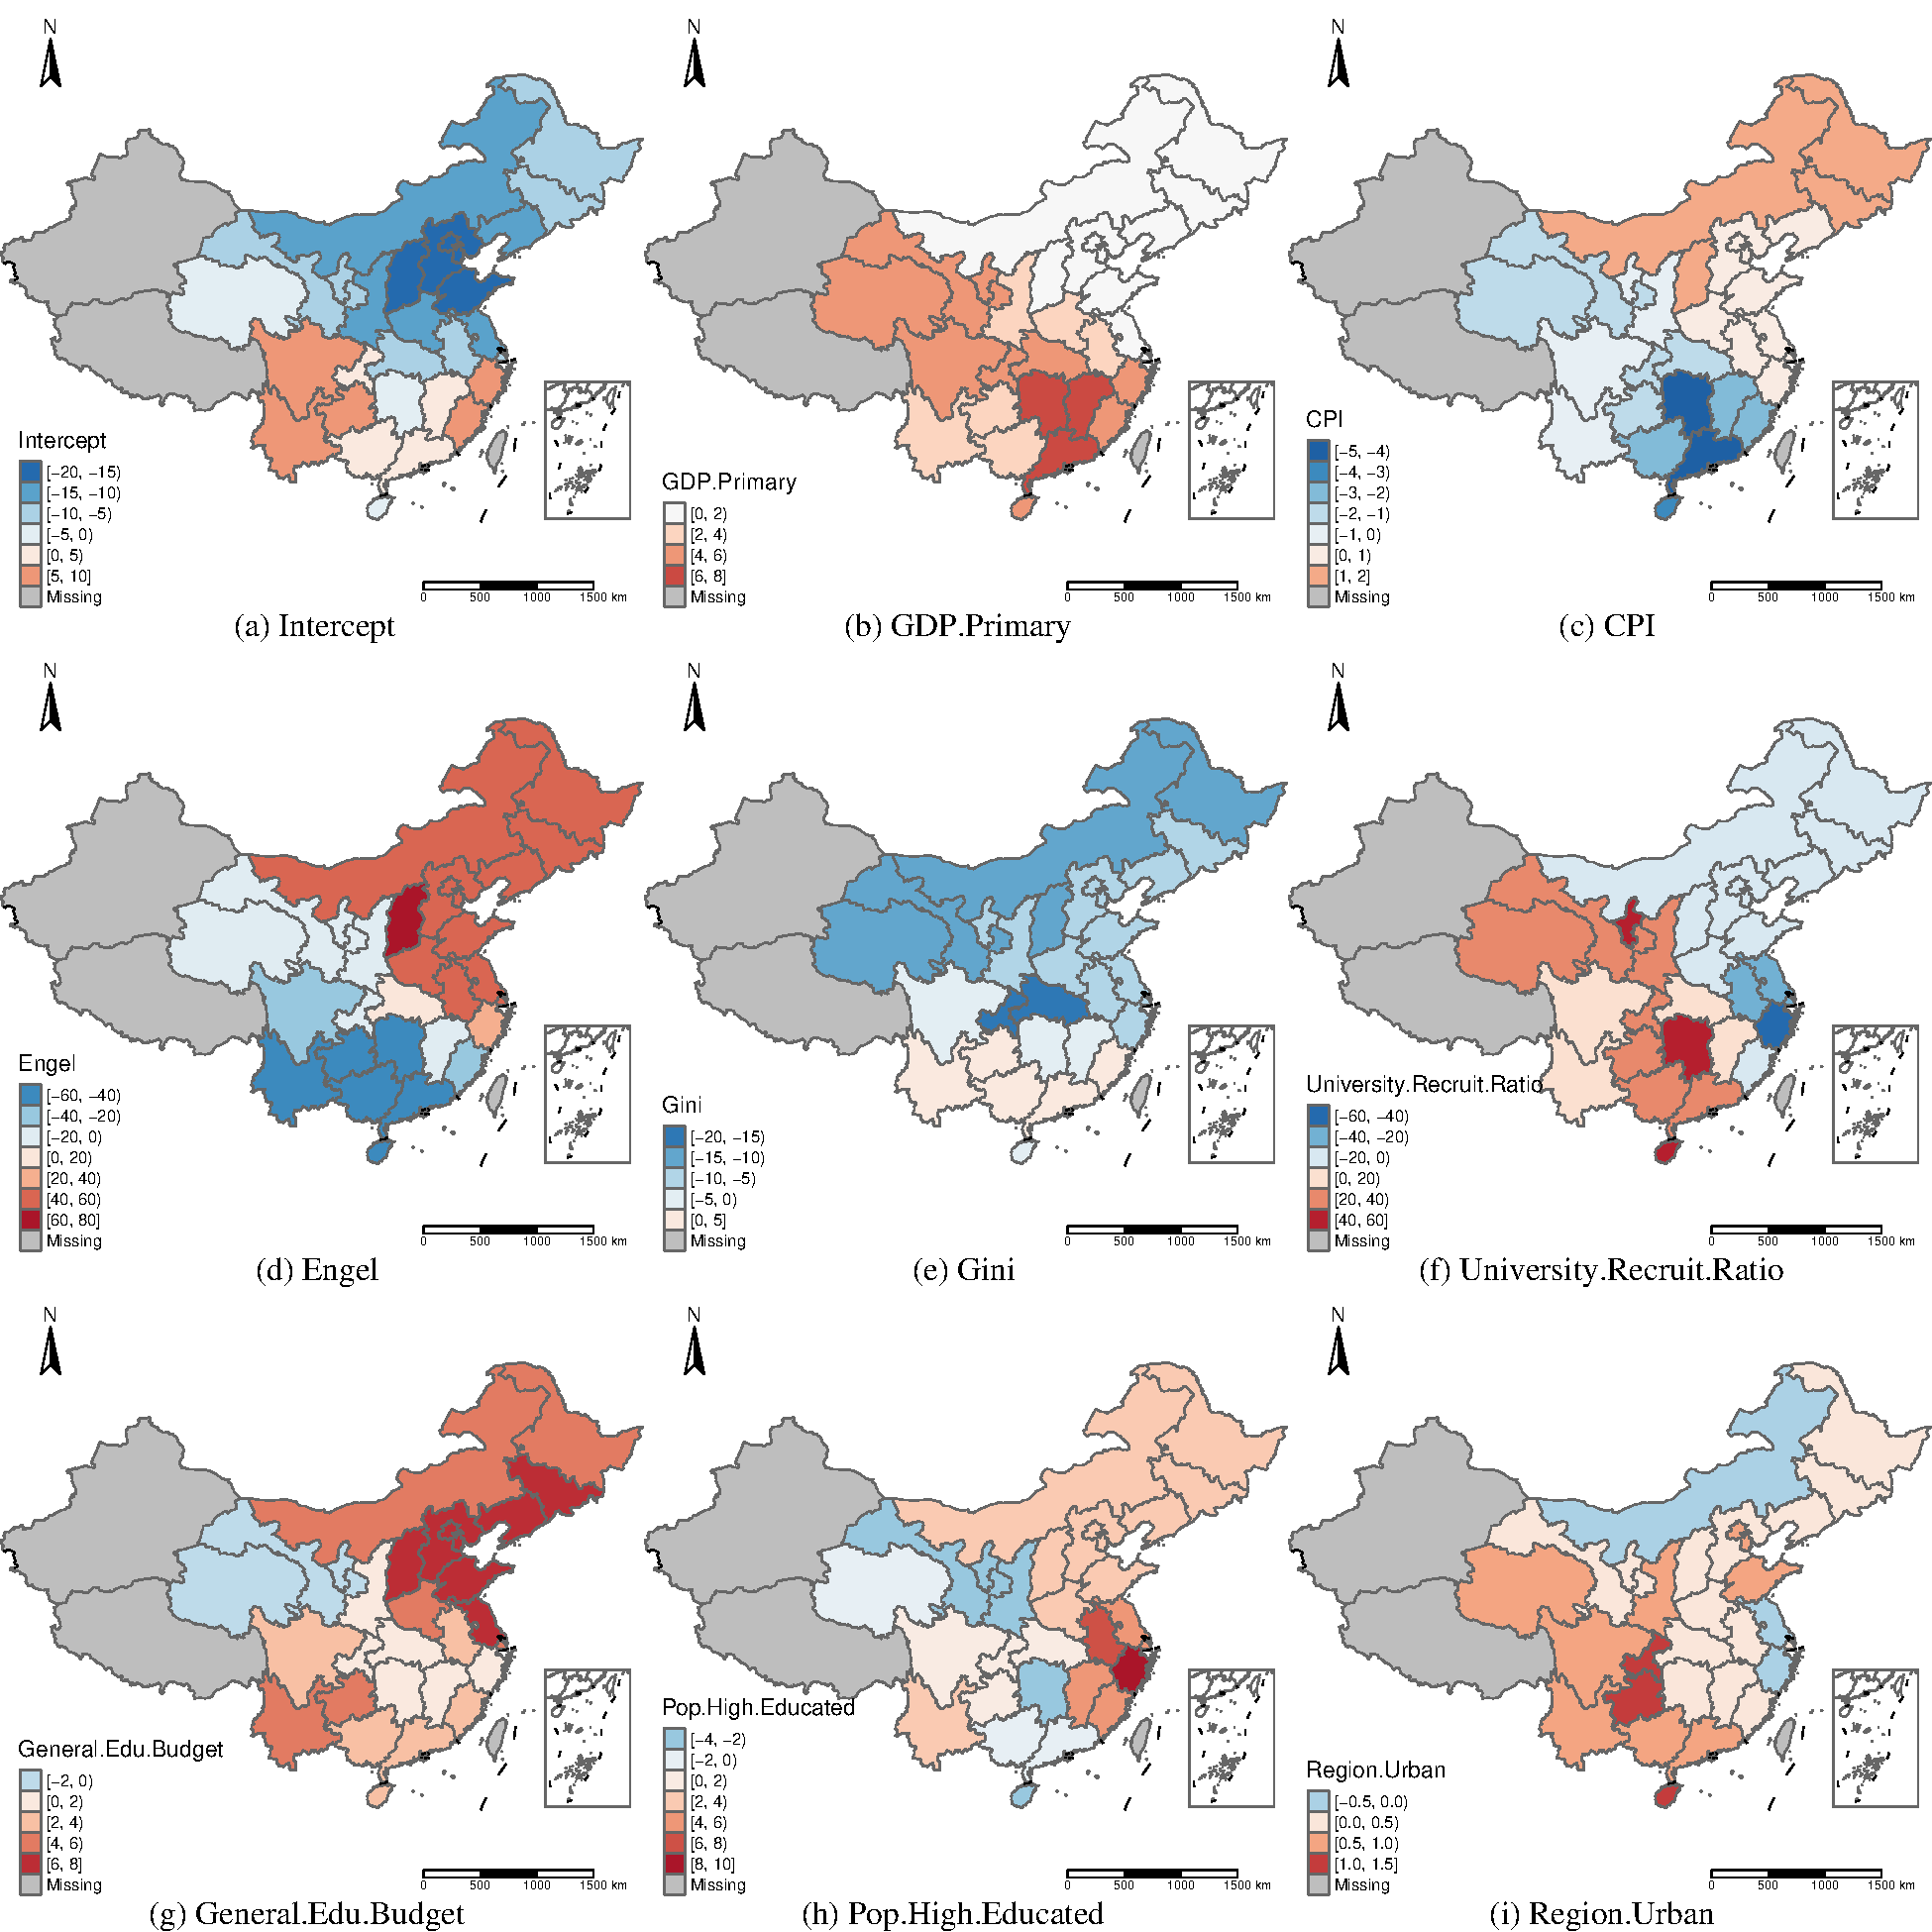
\includegraphics[width=\textwidth]{fig/fig_SpendRatio_coef.pdf}
  \caption{Coefficient estimates from the alternative model.}
  \label{fig:modelratio-coef-glsw-slr}
\end{figure}
\end{document}
